\subsection{Ansible}
In computing, Ansible is an open-source software provisioning, configuration management, and application deployment tool. It runs on many Unix-like systems, and can configure both Unix-like systems as well as Microsoft Windows. It includes its own declarative language to describe system configuration.

Our aim is to deploy our entire application with its dependencies and infrastructure using single executable script. This process of deploying using single executable script is shown in Figure \ref{fig:cloudansibledeplyment}.

\begin{figure}[H]
    \centering
    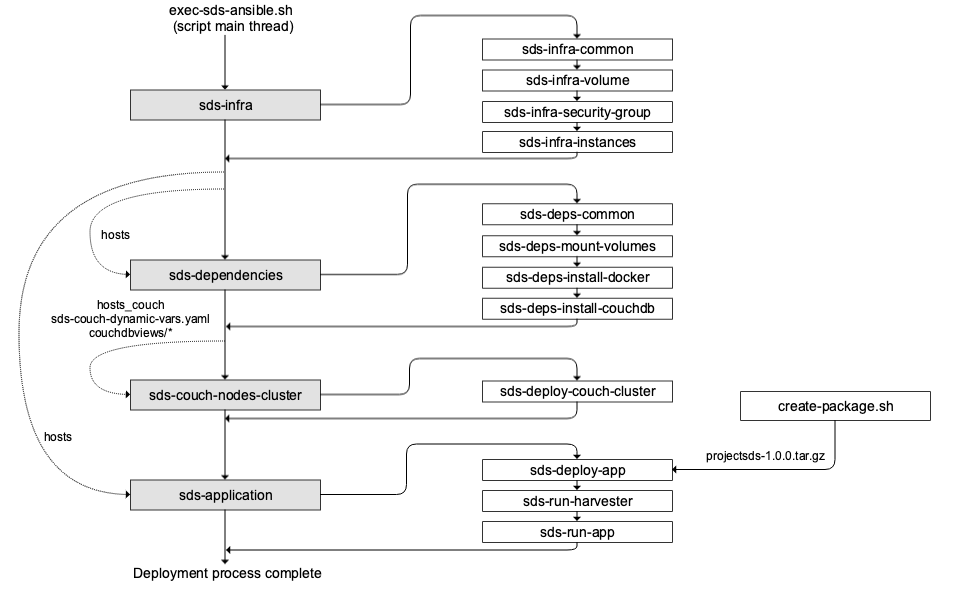
\includegraphics[width=16cm,keepaspectratio=true]{images/deployment/cloud_deployment_ansible.png}
    \caption{Cloud deployment process flow (Ansible)}
    \label{fig:cloudansibledeplyment}
\end{figure}

Using this ansible package, we can deploy application with all its the dependencies and required infrastructure. It follows a serial execution flow to deploy all functionalities.

\subsubsection{Infrastructure}
\textbf{sds-infra:} This ansible package is used to deploy all the required infrastructure related aspects of the application. This package use \emph{sds-infra-vars.yaml} script to provide configuration for the below roles, which are explained in their respective execution order:

\textbf{- sds-infra-common:} This role will install required common dependencies for building infrastructure such as python-pip and openstacksdk.

\textbf{- sds-infra-volume:} This role will create volumes on the cloud as per the names provided and map their ids with name in a dictionary.

\textbf{ - sds-infra-security-group:} This role will create required security groups with their rules on the cloud.

\textbf{ - sds-infra-instances:} This role will create required VM instances and map above created volumes and security groups with their respective instances as shown in Figure \ref{fig:createinstance}, which is then executed by \emph{os\_server}.

After these roles are executed successfully, the main control execution script - \emph{exec-sds-ansible.sh} - transfers the dynamic files generated by \emph{sds-infra} depending upon the role requirement:

\textbf{- hosts:} This file contains IPv4 addresses of successfully installed virtual machines. It is transferred to \emph{sds-dependencies} and \emph{sds-application} package for installing dependencies and deploying application on these web servers.

\textbf{ - hosts\_couch:} This file contains IPv4 address of the virtual machine which will be targeted as the master node for establishing connections and performing handshakes with the other couch nodes. 

\textbf{ - sds-couch-dynamic-vars.yaml:} This file contains IPv4 addresses of the virtual machines which will be targeted as the slave couch nodes for becoming part of the couch cluster initiated by the master node.


\subsubsection{Dependencies}
\textbf{sds-dependencies:} This ansible package is used to install all the required dependencies on the virtual machines created by \emph{sds-infra} package. 
This package use \emph{sds-deps-vars.yaml} script to provide configuration for the below roles with dynamically generated and transferred \emph{hosts} file, which are explained in their respective execution order:

\textbf{-sds-deps-common:} This role will install basic dependencies which is required by the application on the newly created VM hosts.

\textbf{-sds-deps-mount-volumes:} This role will format the volumes to ext4 filesystem on the VMs and mount them on the location as provided using configuration.

\textbf{-sds-deps-install-docker:} This role will install docker on all the provided host VMs by setting proper repositories for downloading and installing docker. This provides ability to build and run docker containers on all VMs which is used by harvester and application as explained in Section \ref{docker}.

\textbf{-sds-deps-install-couchdb:} This role will install CouchDB 2.0 on all the host VMs provided, by configuring and building it from the source and installing it on external mounted storage. 
\newline
\newline
\textbf{sds-couch-nodes-cluster:} This ansible package will enable CouchDB cluster on all the couchdb nodes installed by the previous package. This package uses curl commands to register nodes in the cluster and starting cluster after proper setup, which is then followed by database and view initilization in multi-node environment as explained in Section \ref{couchdb}.

This package depends on 2 dynamically created files by sds-infra package - \emph{hosts\_couch} and \emph{sds-couch-dynamic-vars.yaml} and uses static custom \emph{json} files to create views inside the database. As explained above, both of these files and couchdb views are transferred to their proper locations by the main control script: \texttt{exec-sds-ansible.sh}

\textbf{-sds-deploy-couch-cluster:} This role will enable CouchDB cluster using the host provided in \emph{hosts\_couch} file and registering all other nodes in the cluster as per the dynamic configuration.

\subsubsection{Application}
\textbf{sds-application:} This ansible package is used to deploy and install the application with harvester on the virtual machines created by \emph{sds-infra} package. Before starting roles of this package, we use custom created script - \texttt{create\_package.sh} - which transforms our entire project into \texttt{.tar.gz} file and copy package into required location, which can later be deployed and extracted in VMs using following roles:

\textbf{-sds-deploy-app:} This role will create the project directory in all provided VMs, deploy \texttt{.tar.gz} package and unarchive it using ansible commands.

\textbf{-sds-run-harvester:} This role starts the harvester by building docker image and starting container. Before building image, it uses ansible \texttt{regexp} for pointing harvester's configuration to correct couchdb as shown in Figure \ref{fig:couchharvester}.

\begin{figure}[H]
    \centering
    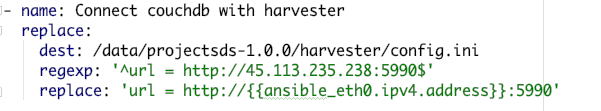
\includegraphics[width=10cm,keepaspectratio=true]{images/deployment/couch_harvester.png}
    \caption{Connecting appropriate couchdb with harvester}
    \label{fig:couchharvester}
\end{figure}

\textbf{-sds-run-app:} This role starts the application python \texttt{flask} server which exposes API endpoints for UI interactions and manipulations. It is also started by building docker image and starting container. Similar to above \texttt{regexp} code, application data connector configuration is also pointed to correct couch db.

\begin{figure}[H]
    \centering
    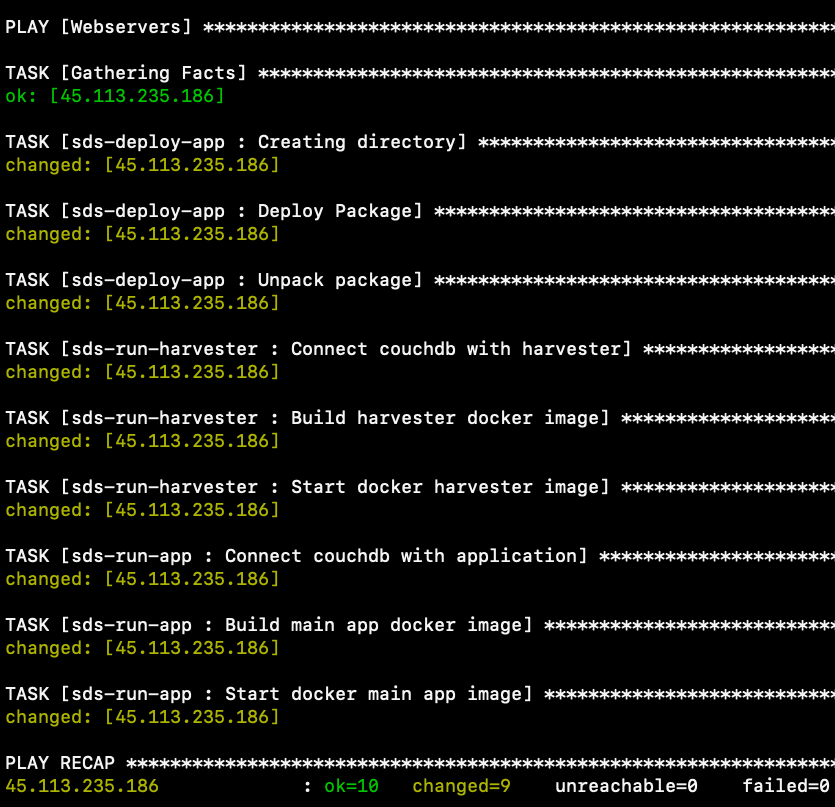
\includegraphics[width=10cm,keepaspectratio=true]{images/deployment/app_deployment_ansible.png}
    \caption{\texttt{sds-application} ansible deployment flow}
    \label{fig:appansibledeplyment}
\end{figure}
